% !TeX program = pdflatex
\documentclass[11pt,a4paper]{report}

\usepackage[margin=23mm]{geometry}
\usepackage[T5,T1]{fontenc}
\usepackage[utf8]{inputenc}
\usepackage[vietnamese,english]{babel}
\usepackage{lmodern}
\usepackage{microtype}
\usepackage{graphicx}
\usepackage{booktabs}
\usepackage{array}
\usepackage{tabularx}
\usepackage{amsmath,amssymb}
\usepackage{float}
\usepackage{subcaption}
\usepackage{xcolor}
\usepackage{enumitem}
\usepackage{fancyhdr}
\usepackage{hyperref}
\usepackage{placeins}

\graphicspath{{assets/}}
\hypersetup{colorlinks=true,linkcolor=blue!55!black,citecolor=blue!55!black,urlcolor=blue!55!black}
\setlength{\parindent}{0pt}
\setlength{\parskip}{5pt}
\setcounter{secnumdepth}{3}
\setcounter{tocdepth}{2}

\definecolor{navy}{RGB}{25,56,92}
\definecolor{lightblue}{RGB}{229,239,249}
\definecolor{passgreen}{RGB}{0,105,70}
\definecolor{failred}{RGB}{170,35,35}
\definecolor{warnorange}{RGB}{185,105,0}

\pagestyle{fancy}
\fancyhf{}
\fancyhead[L]{\scriptsize\itshape\foreignlanguage{vietnamese}{Trường Đại học Khoa học Tự nhiên - Khoa Điện tử - Viễn thông}}
\fancyhead[R]{\scriptsize\itshape\foreignlanguage{vietnamese}{Lê Phan Thanh Liêm}}
\fancyfoot[C]{\thepage}
\renewcommand{\headrulewidth}{0.4pt}
\fancypagestyle{plain}{%
  \fancyhf{}
  \fancyhead[L]{\scriptsize\itshape\foreignlanguage{vietnamese}{Trường Đại học Khoa học Tự nhiên - Khoa Điện tử - Viễn thông}}
  \fancyhead[R]{\scriptsize\itshape\foreignlanguage{vietnamese}{Lê Phan Thanh Liêm}}
  \fancyfoot[C]{\thepage}
  \renewcommand{\headrulewidth}{0.4pt}}

\newcommand{\V}{\mathrm{V}}
\newcommand{\A}{\mathrm{A}}
\newcommand{\Hz}{\mathrm{Hz}}
\newcommand{\dd}{\mathrm{d}}
\newcommand{\micro}{\mu}
\newcommand{\ohm}{\Omega}
\newcommand{\SI}[2]{\ensuremath{#1\,\mathrm{#2}}}
\newcommand{\si}[1]{\ensuremath{\mathrm{#1}}}
\newcommand{\SIrange}[3]{\ensuremath{#1\text{--}#2\,\mathrm{#3}}}
\newcommand{\ang}[1]{\ensuremath{#1^{\circ}}}
\newcommand{\pass}{\textcolor{passgreen}{Pass}}
\newcommand{\fail}{\textcolor{failred}{Not met}}
\newcommand{\pending}{\textcolor{warnorange}{Re-test}}
\newcommand{\figwide}[3][0.96\textwidth]{%
  \begin{figure}[H]\centering
  \includegraphics[width=#1]{#2}
  \caption{#3}\end{figure}}

\begin{document}

\begin{titlepage}
  \centering
  \vspace*{7mm}
  {\large\bfseries\foreignlanguage{vietnamese}{TRƯỜNG ĐẠI HỌC KHOA HỌC TỰ NHIÊN - ĐHQG TP.HCM}\par}
  \vspace{1.5mm}
  {\large\bfseries\foreignlanguage{vietnamese}{KHOA ĐIỆN TỬ - VIỄN THÔNG}\par}
  \vspace{7mm}
  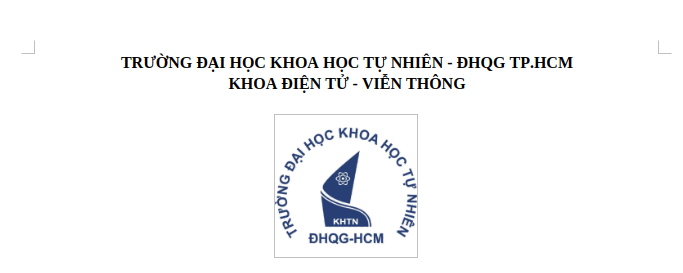
\includegraphics[width=31mm,trim=270 14 270 112,clip]{khtn_reference.png}\par
  \vspace{10mm}
  {\Large\bfseries ADVANCED ANALOG INTEGRATED CIRCUIT DESIGN\par}
  \vspace{8mm}
  {\color{navy}\rule{\textwidth}{1.2pt}\par}
  \vspace{8mm}
  {\Huge\bfseries Design and Analysis of a Two-Stage Miller-Compensated CMOS Operational Amplifier\par}
  \vspace{7mm}
  {\Large GPDK090, \SI{1.2}{V} Supply\par}
  \vspace{8mm}
  {\color{navy}\rule{\textwidth}{1.2pt}\par}
  \vfill
  \begin{tabular}{rl}
    \textbf{Student:} & \foreignlanguage{vietnamese}{Lê Phan Thanh Liêm}\\
    \textbf{Design environment:} & Cadence Virtuoso / Spectre\\
    \textbf{Technology:} & GPDK090 BSIM3\\
    \textbf{Date:} & October 2026
  \end{tabular}
  \vfill
  {\small This report separates hand calculations, transistor-level operating-point checks, and simulation measurements. Values not directly demonstrated by the available plots are explicitly marked as estimates or re-test items.\par}
\end{titlepage}

\pagenumbering{roman}
\chapter*{Abstract}
\addcontentsline{toc}{chapter}{Abstract}
This report presents the hand design and transistor-level verification of an unbuffered, two-stage CMOS operational amplifier with Miller compensation. The circuit uses an NMOS differential input pair, a PMOS current-mirror active load, an NMOS tail source, a PMOS common-source second stage, and an NMOS sink load. The nominal supply is \SI{1.2}{V}; the external load is \SI{10}{pF}; the selected Miller capacitor is \SI{3.6}{pF}; and the bias reference is \SI{6.1}{\micro A}.

The design was initially sized for a target dc gain of at least \SI{70}{dB}, a gain-bandwidth product of \SI{5}{MHz}, a slew rate of \SI{5}{V/\micro s}, an input common-mode range of \SIrange{0.4}{0.9}{V}, and approximately \ang{60} phase margin. Spectre simulation gives \SI{74.05}{dB} low-frequency open-loop gain, a \SI{851.14}{Hz} dominant-pole bandwidth, a near-unity-gain frequency of approximately \SI{3.72}{MHz}, and approximately \ang{54.3} phase margin. The simulated 1\% settling times are about \SI{0.22}{\micro s} and \SI{0.25}{\micro s} for positive and negative steps. The low-frequency CMRR, PSRR$^+$, and PSRR$^-$ are approximately \SI{79.62}{dB}, \SI{85.75}{dB}, and \SI{84.13}{dB}, respectively.

\tableofcontents
\clearpage
\pagenumbering{arabic}

\chapter{Introduction and Design Requirements}

\section{Objective}
The objective is to design, size, and verify a compact two-stage CMOS operational amplifier in the GPDK090 process. The report follows a calculation-first flow: analytical equations establish a first-cut design, dc operating-point data checks bias and saturation, ac analysis evaluates gain and stability, and transient analysis evaluates large-signal speed and settling. The design method and small-signal interpretation follow the standard treatments of analog CMOS design in Razavi and Baker \cite{razavi,baker}, together with the unbuffered two-stage design procedure summarized by Allen \cite{allen}.

\section{Architecture}
The transistor functions are:
\begin{itemize}[leftmargin=18mm]
  \item M1--M2: matched NMOS differential input pair;
  \item M3--M4: matched PMOS current-mirror load and single-ended conversion;
  \item M5: NMOS tail-current source;
  \item M6: PMOS common-source second gain stage;
  \item M7: NMOS output-stage current sink, implemented with multiplicity $m=6$;
  \item M8: diode-connected NMOS device that converts $I_{BIAS}$ into the bias voltage for M5 and M7;
  \item $C_C$: Miller compensation capacitor from the first-stage output to the amplifier output.
\end{itemize}

\figwide[0.89\textwidth]{dc_operating.png}{Final transistor-level schematic with dc node voltages and device dimensions.}

\section{Target specifications and design constants}
\begin{table}[H]
\centering
\caption{Design targets and fixed conditions.}
\begin{tabularx}{\textwidth}{>{\bfseries}l >{\raggedright\arraybackslash}X l}
\toprule
Parameter & Target / selected value & Symbol\\
\midrule
Supply rails & $V_{DD}=\SI{1.2}{V}$, $V_{SS}=\SI{0}{V}$ & $V_{DD},V_{SS}$\\
DC open-loop gain & at least \SI{70}{dB} & $A_0$\\
Gain-bandwidth product & \SI{5}{MHz} & GBW\\
Phase margin & approximately \ang{60} or higher & PM\\
Load capacitance & \SI{10}{pF} & $C_L$\\
Miller capacitance & \SI{3.6}{pF} & $C_C$\\
Slew rate & \SI{5}{V/\micro s} & SR\\
1\% settling time & at most \SI{1}{\micro s} for a \SI{0.4}{V} step & $t_s$\\
Input common-mode range & \SIrange{0.4}{0.9}{V} & ICMR\\
Bias reference & \SI{6.1}{\micro A} & $I_{BIAS}$\\
Process transconductance parameters & $K_n'=\SI{296.4}{\micro A/V^2}$, $K_p'=\SI{167.4}{\micro A/V^2}$ & $K_n',K_p'$\\
\bottomrule
\end{tabularx}
\end{table}

The threshold values used in the first-cut sizing are extracted from the design work: $|V_{TP}|_{max}=\SI{0.149135}{V}$, $V_{TN,min}=\SI{0.151885}{V}$, and $V_{TN,max}=\SI{0.186604}{V}$. These simplified values are used only for hand sizing; Spectre uses the complete BSIM3 model.

\chapter{First-Cut Analytical Design}

\section{Design relations}
For $S_i=(W/L)_i$ and matched mirror devices, the principal relations are
\begin{align}
SR &\approx \frac{I_5}{C_C},\\
GBW &\approx \frac{g_{m1}}{2\pi C_C},\\
A_{v1} &\approx \frac{g_{m2}}{g_{ds2}+g_{ds4}},\\
A_{v2} &\approx \frac{g_{m6}}{g_{ds6}+g_{ds7}},\\
A_0 &\approx A_{v1}A_{v2},\\
p_2 &\approx -\frac{g_{m6}}{C_L},\qquad
z_{RHP}\approx \frac{g_{m6}}{C_C}.
\end{align}
For the classical Miller-compensated topology without a nulling resistor, a practical \ang{60} phase-margin rule is
\begin{equation}
g_{m6}\approx 2.2\,g_{m2}\frac{C_L}{C_C},
\end{equation}
provided that other high-frequency poles are well above the unity-gain frequency.

\section{Compensation capacitor and tail current}
The minimum compensation capacitor from the design rule is
\begin{equation}
C_C>0.22C_L=0.22(\SI{10}{pF})=\SI{2.2}{pF}.
\end{equation}
The selected value $C_C=\SI{3.6}{pF}$ provides additional pole separation. From the slew-rate target,
\begin{equation}
I_5=SR\,C_C=(\SI{5}{V/\micro s})(\SI{3.6}{pF})=\boxed{\SI{18}{\micro A}}.
\end{equation}

\section{Input pair and PMOS mirror}
The required input-pair transconductance is
\begin{equation}
g_{m1}=2\pi(GBW)C_C=2\pi(\SI{5}{MHz})(\SI{3.6}{pF})
=\boxed{\SI{113.10}{\micro S}}.
\end{equation}
At $V_{in,max}=\SI{0.9}{V}$, the mirror overdrive used for the first cut is
\begin{align}
V_{OV3}&=V_{DD}-V_{in,max}-|V_{TP}|_{max}+V_{TN,min}\\
&=1.2-0.9-0.149135+0.151885=\SI{0.30275}{V}.
\end{align}
Therefore,
\begin{equation}
S_3=S_4=\frac{I_5}{K_p'V_{OV3}^2}=\boxed{1.173}.
\end{equation}
For M1 and M2,
\begin{equation}
S_1=S_2=\frac{g_{m1}^2}{K_n'I_5}=\boxed{2.397}.
\end{equation}

\section{Tail transistor M5}
The input-pair overdrive from the first-cut values is
\begin{equation}
V_{OV1}=\sqrt{\frac{I_5}{K_n'S_1}}=\SI{0.15915}{V}.
\end{equation}
A conservative hand calculation used $V_{in,min}=\SI{0.45}{V}$ to keep finite saturation margin:
\begin{align}
V_{DS5,sat}&=V_{in,min}-V_{SS}-V_{OV1}-V_{TN,max}\\
&=0.45-0.15915-0.186604=\SI{0.10424}{V},\\
S_5&=\frac{2I_5}{K_n'V_{DS5,sat}^2}=\boxed{11.178}.
\end{align}
This conservative equation predicts a lower ICMR near \SI{0.45}{V}. The requested \SI{0.4}{V} lower limit must therefore be verified by the transistor model rather than assumed from the square-law estimate.

\section{Second stage M6 and output sink M7}
The PMOS mirror transconductance estimated from the first stage is
\begin{equation}
g_{m4}=\frac{I_5}{V_{OV3}}=\SI{59.45}{\micro S}.
\end{equation}
The transconductance required for approximate \ang{60} phase margin is
\begin{equation}
g_{m6}=2.2g_{m2}\frac{C_L}{C_C}
=2.2(\SI{113.10}{\micro S})\frac{10}{3.6}
=\boxed{\SI{691.15}{\micro S}}.
\end{equation}
Using the matched-mirror relationship,
\begin{align}
S_6&=\frac{g_{m6}}{g_{m4}}S_4=\boxed{13.637},\\
I_6&=\frac{g_{m6}^2}{2K_p'S_6}=\boxed{\SI{104.62}{\micro A}},\\
S_7&=\frac{I_6}{I_5}S_5=\boxed{64.968}.
\end{align}

\section{Bias device M8}
M8 and M5 share the same gate-source voltage. Hence their drain currents scale with geometry:
\begin{equation}
\frac{I_{BIAS}}{I_5}=\frac{S_8}{S_5}quad\Rightarrow\quad
S_8=S_5\frac{I_{BIAS}}{I_5}
=11.178\frac{6.1}{18}=\boxed{3.788}.
\end{equation}
With $L_8=\SI{1.44}{\micro m}$, the calculated width is $W_8=\SI{5.45}{\micro m}$, which is the implemented value.

\section{First-cut and implemented dimensions}
\begin{table}[H]
\centering
\caption{Calculated sizing and dimensions used in the final schematic.}
\begin{tabular}{cccccc}
\toprule
Device & Calculated $S=W/L$ & First-cut $W$ & Final $W$ & Final $L$ & Multiplicity\\
& & (\si{\micro m}) & (\si{\micro m}) & (\si{\micro m}) & $m$\\
\midrule
M1, M2 & 2.397 & 2.59 & 2.60 & 1.08 & 1\\
M3, M4 & 1.173 & 1.27 & 1.26 & 1.08 & 1\\
M5 & 11.178 & 16.10 & 16.10 & 1.44 & 1\\
M6 & 13.637 & 19.64 & 19.63 & 1.44 & 1\\
M7 & 64.968 effective & 15.59 per finger & 15.30 & 1.44 & 6\\
M8 & 3.788 & 5.45 & 5.45 & 1.44 & 1\\
\bottomrule
\end{tabular}
\end{table}
The implemented dimensions preserve the calculated ratios while using practical channel lengths and multiplicity. M7 was rounded slightly during dc balancing. Such small tuning is expected because the square-law equations neglect channel-length modulation, body effect, mobility degradation, and intrinsic capacitances.

The idealized quiescent power estimate is
\begin{equation}
P_{DC}\approx V_{DD}(I_5+I_6+I_{BIAS})
=1.2(18+104.62+6.1)\,\si{\micro A}
=\boxed{\SI{154.5}{\micro W}}.
\end{equation}
This is an analytical estimate; the final report should use the Spectre supply-current measurement if an exact power value is required.

\chapter{DC Analysis}

\section{Operating-point verification}
The dc operating point was evaluated at $V_{IN+}=V_{IN-}=\SI{0.6}{V}$ with $C_L=\SI{10}{pF}$. The schematic reports $V_{OUT}\approx\SI{0.598}{V}$ and every device is marked in region 2, which is the simulator's saturation-region code for these MOS models.

\figwide[0.84\textwidth]{dc_operating.png}{Annotated dc operating point at $V_{IN+}=V_{IN-}=\SI{0.6}{V}$. The displayed node voltages make the headroom and stage balance directly visible.}

\begin{samepage}
The annotated schematic supports the following dc checks:
\begin{itemize}[leftmargin=18mm,itemsep=2pt]
  \item The two input gates are both at \SI{0.6}{V}, while the common-source node of M1--M2 is approximately \SI{0.2338}{V}. The differential pair is therefore biased symmetrically.
  \item The two first-stage drain nodes are approximately \SI{0.6929}{V} and \SI{0.7006}{V}. Their small difference is consistent with the single-ended current-mirror conversion and device-model nonidealities.
  \item The M5 drain voltage is approximately \SI{0.2338}{V}, which is greater than its recorded $V_{DS,sat}\approx\SI{0.100}{V}$. M5 therefore retains about \SI{0.134}{V} saturation margin.
  \item The bias node shared by M8, M5, and M7 is approximately \SI{0.273}{V}. The close agreement between the intended \SI{6.1}{\micro A} reference and the recorded M8 current confirms the bias-mirror scaling.
  \item The M6 gate voltage is approximately \SI{0.7006}{V}, and $V_{OUT}=\SI{0.5979}{V}$. Consequently, M6 has $V_{SD6}\approx\SI{0.602}{V}$ and M7 has $V_{DS7}\approx\SI{0.598}{V}$, providing comfortable output-stage saturation headroom at the quiescent point.
  \item The output is only about \SI{2.1}{mV} below the ideal mid-supply value of \SI{0.6}{V}, showing that the final M6--M7 current balance is well centered.
\end{itemize}
\end{samepage}

\figwide[0.98\textwidth]{op_table.jpeg}{Recorded Spectre operating-point quantities for M1--M8.}

The most useful quantities transcribed from the operating-point record are summarized below. Handwritten last digits are rounded; conclusions should rely on their order of magnitude rather than the final digit.
\begin{table}[H]
\centering
\caption{Selected nominal operating-point data.}
\begin{tabular}{crrrcc}
\toprule
Device & $I_D$ & $g_m$ & $g_{ds}$ & Region & $|V_{DS}|$\\
\midrule
M1 & \SI{8.893}{\micro A} & \SI{101.43}{\micro S} & \SI{6.26}{nS} & 2 & \SI{0.959}{V}\\
M2 & \SI{8.898}{\micro A} & \SI{101.48}{\micro S} & \SI{6.21}{nS} & 2 & \SI{0.487}{V}\\
M3 & \SI{8.892}{\micro A} & \SI{46.48}{\micro S} & \SI{467.24}{nS} & 2 & \SI{0.507}{V}\\
M4 & \SI{8.83}{\micro A} & \SI{46.45}{\micro S} & \SI{480.29}{nS} & 2 & \SI{0.499}{V}\\
M5 & \SI{17.79}{\micro A} & \SI{282.5}{\micro S} & \SI{1.73}{\micro S} & 2 & \SI{0.234}{V}\\
M6 & \SI{103.82}{\micro A} & \SI{551.0}{\micro S} & \SI{3.65}{\micro S} & 2 & \SI{0.602}{V}\\
M7 & \SI{103.82}{\micro A} & \SI{1.60}{mS} & \SI{5.78}{\micro S} & 2 & \SI{0.598}{V}\\
M8 & \SI{6.09}{\micro A} & \SI{96.49}{\micro S} & \SI{0.464}{\micro S} & 2 & \SI{0.273}{V}\\
\bottomrule
\end{tabular}
\end{table}

The current checks are consistent with the intended biasing:
\begin{equation}
I_{D1}+I_{D2}=\SI{17.791}{\micro A}\approx I_{D5}=\SI{17.79}{\micro A},
\end{equation}
and
\begin{equation}
I_{D6}\approx I_{D7}\approx\SI{103.82}{\micro A}.
\end{equation}

\section{Gain estimated from the dc operating point}
Using the measured small-signal parameters,
\begin{align}
A_{v1}&\approx\frac{101.475\,\si{\micro S}}
{6.21\,\si{nS}+480.291\,\si{nS}}
=208.6\quad(\SI{46.39}{dB}),\\
A_{v2}&\approx\frac{550.997\,\si{\micro S}}
{3.649\,\si{\micro S}+5.78\,\si{\micro S}}
=58.44\quad(\SI{35.33}{dB}),\\
A_{0,OP}&\approx A_{v1}A_{v2}=1.219\times10^4
\quad(\SI{81.72}{dB}).
\end{align}
The full ac simulation gives \SI{74.05}{dB}. The approximately \SI{7.7}{dB} difference shows the limit of multiplying two isolated $g_m/g_{ds}$ stage estimates. The complete model includes loading between stages, body transconductance, frequency-dependent intrinsic elements, and the finite impedances of bias networks.

\section{Input common-mode range}
The ICMR testbench connects the amplifier as a unity-gain follower and sweeps the common-mode input. The tracking error is
\begin{equation}
e_{CM}=V_{OUT}-V_{CM}.
\end{equation}

\figwide[0.76\textwidth]{tb_icmr.png}{Unity-gain follower testbench used for the ICMR sweep.}
\figwide[0.82\textwidth]{icmr_max.png}{Upper ICMR sweep. The marked point is $V_{CM}=\SI{0.9575}{V}$ with approximately \SI{3.12}{mV} tracking error.}

The upper boundary is therefore approximately \SI{0.958}{V} under the shown error criterion, so the required \SI{0.9}{V} upper limit is satisfied. The theoretical design boundary was \SI{0.9}{V}; the nominal transistor model provides some extra margin.

\figwide[0.82\textwidth]{icmr_min.png}{Available lower-bound plot. The horizontal axis is displayed in millivolts and spans only 0--\SI{3}{mV}; therefore this plot does not validate a \SI{0.4}{V} lower ICMR limit.}

The conservative square-law estimate is
\begin{equation}
V_{ICMR,min}\approx V_{SS}+V_{OV1}+V_{TN,max}+V_{DS5,sat}
=0+0.1592+0.1866+0.1042\approx\SI{0.450}{V}.
\end{equation}
Consequently, the lower ICMR is reported as \emph{not yet signed off}. The dc sweep must be repeated over, for example, \SIrange{0.2}{0.6}{V}, not \SIrange{0}{3}{mV}. The target interval \SIrange{0.4}{0.9}{V} should only be marked as passed if the rerun keeps $|e_{CM}|$ below the chosen limit and all critical devices remain saturated.

\section{Output-voltage swing}
\figwide[0.76\textwidth]{tb_output_swing.png}{DC output-swing testbench. A small differential input sweep drives the open-loop output into both limits.}
\figwide[0.95\textwidth]{output_swing.png}{Output voltage versus differential input near the switching point.}

From the plateaus, the no-load output swing is approximately
\begin{equation}
V_{OUT,min}\approx\SI{0.01}{V},\qquad
V_{OUT,max}\approx\SI{1.10}{V},\qquad
V_{OUT,pp}\approx\SI{1.09}{V}.
\end{equation}
The upper headroom is about \SI{0.10}{V} below $V_{DD}$ and the lower headroom is about \SI{0.01}{V} above $V_{SS}$. This is a dc/no-load result; a resistive load or large output current will reduce the available swing.

\chapter{AC Analysis}

\section{Open-loop gain, bandwidth, and phase margin}
\figwide[0.74\textwidth]{tb_ac.png}{Open-loop differential ac testbench with $C_L=\SI{10}{pF}$ and $C_C=\SI{3.6}{pF}$.}
\figwide[0.98\textwidth]{gain_pm.png}{Open-loop magnitude and phase response.}

The marked measurements are
\begin{align}
A_0&=\SI{74.0526}{dB},\\
f_{-3\,dB}&=\SI{851.138}{Hz},\\
|A(j2\pi f)|&=\SI{0.2896}{dB}\ \text{at}\ f=\SI{3.71535}{MHz},\\
\angle A(j2\pi f)&=-\ang{125.688}\ \text{at}\ f=\SI{3.71535}{MHz}.
\end{align}
The actual 0-dB crossing is slightly above the marked frequency. Using the closest common marker gives
\begin{equation}
f_u\approx\SI{3.72}{MHz},\qquad PM\approx180^\circ-125.688^\circ=\boxed{\ang{54.31}}.
\end{equation}
Thus the design is stable but has less margin than the \ang{60} target. The simulated $g_{m6}\approx\SI{551}{\micro S}$ is lower than the \SI{691}{\micro S} first-cut value, which explains part of the reduced pole separation. The right-half-plane zero created by a bare Miller capacitor also reduces phase margin near unity gain.

\section{Common-mode rejection ratio}
For differential excitation, $v_{in+}=+v_{ac}/2$ and $v_{in-}=-v_{ac}/2$. For common-mode excitation, both inputs receive the same ac signal. The low-frequency CMRR is
\begin{equation}
CMRR_{dB}=A_{d,dB}-A_{cm,dB}.
\end{equation}

\begin{figure}[H]\centering
\begin{subfigure}[t]{0.48\textwidth}\centering
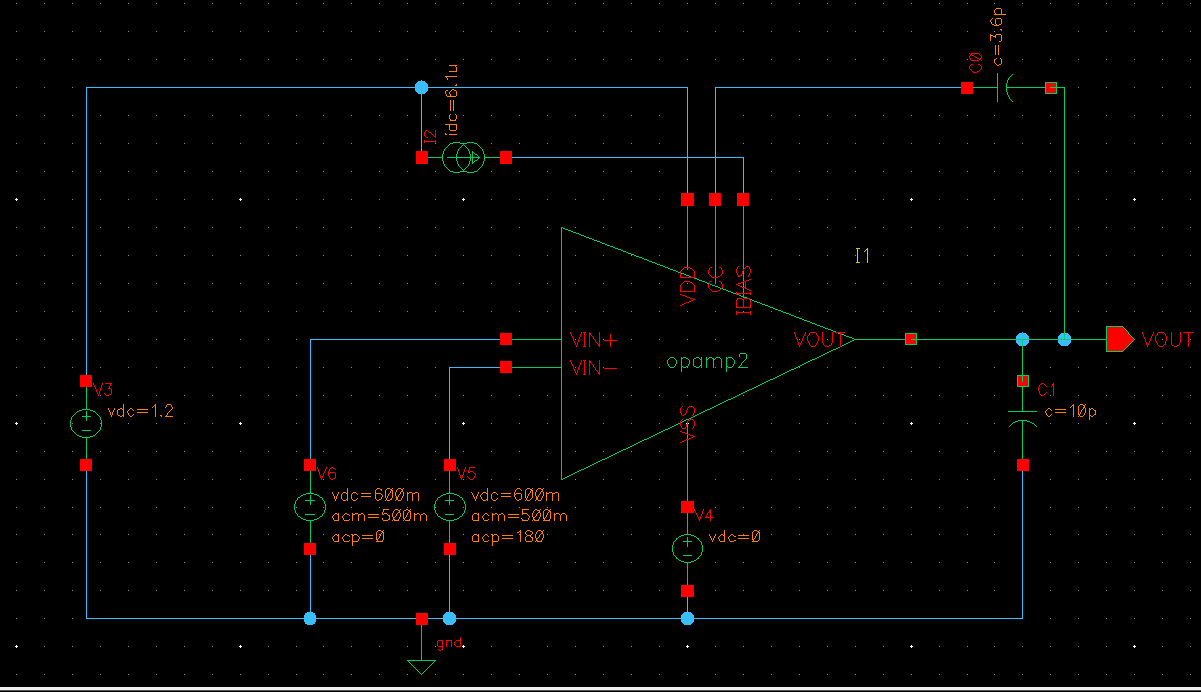
\includegraphics[width=\linewidth]{tb_cmrr_ad.png}
\caption{Differential-gain testbench.}
\end{subfigure}\hfill
\begin{subfigure}[t]{0.48\textwidth}\centering
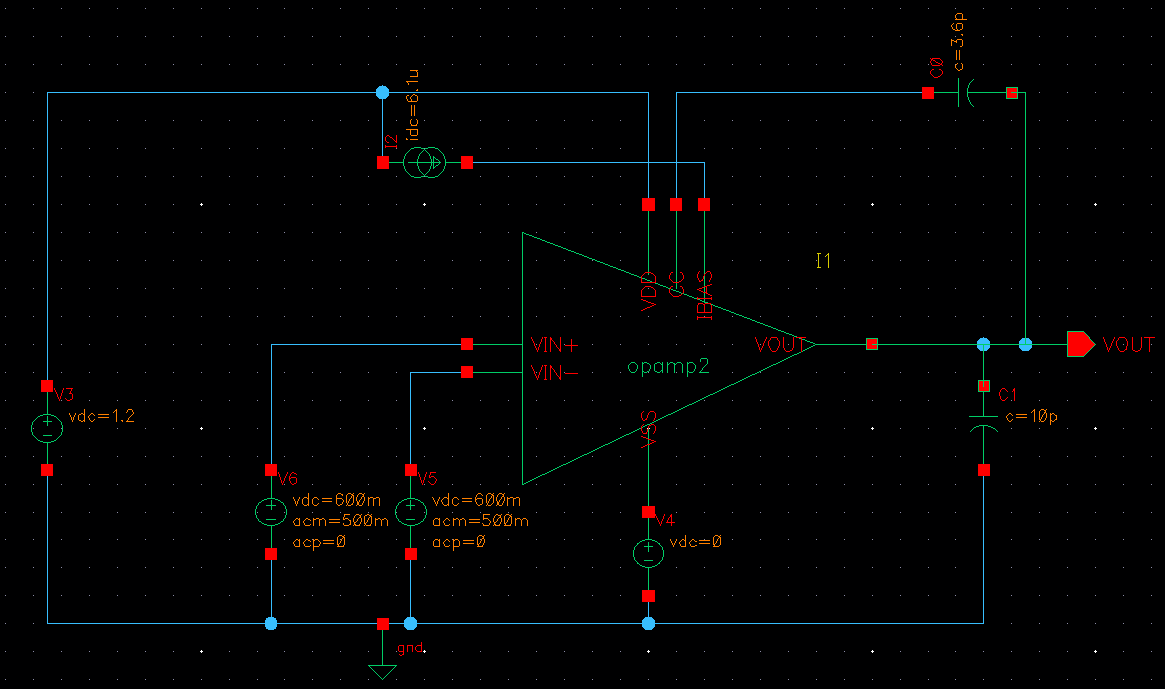
\includegraphics[width=\linewidth]{tb_cmrr_acm.png}
\caption{Common-mode-gain testbench.}
\end{subfigure}
\caption{CMRR test configurations.}
\end{figure}

\begin{figure}[H]\centering
\begin{subfigure}[t]{0.49\textwidth}\centering
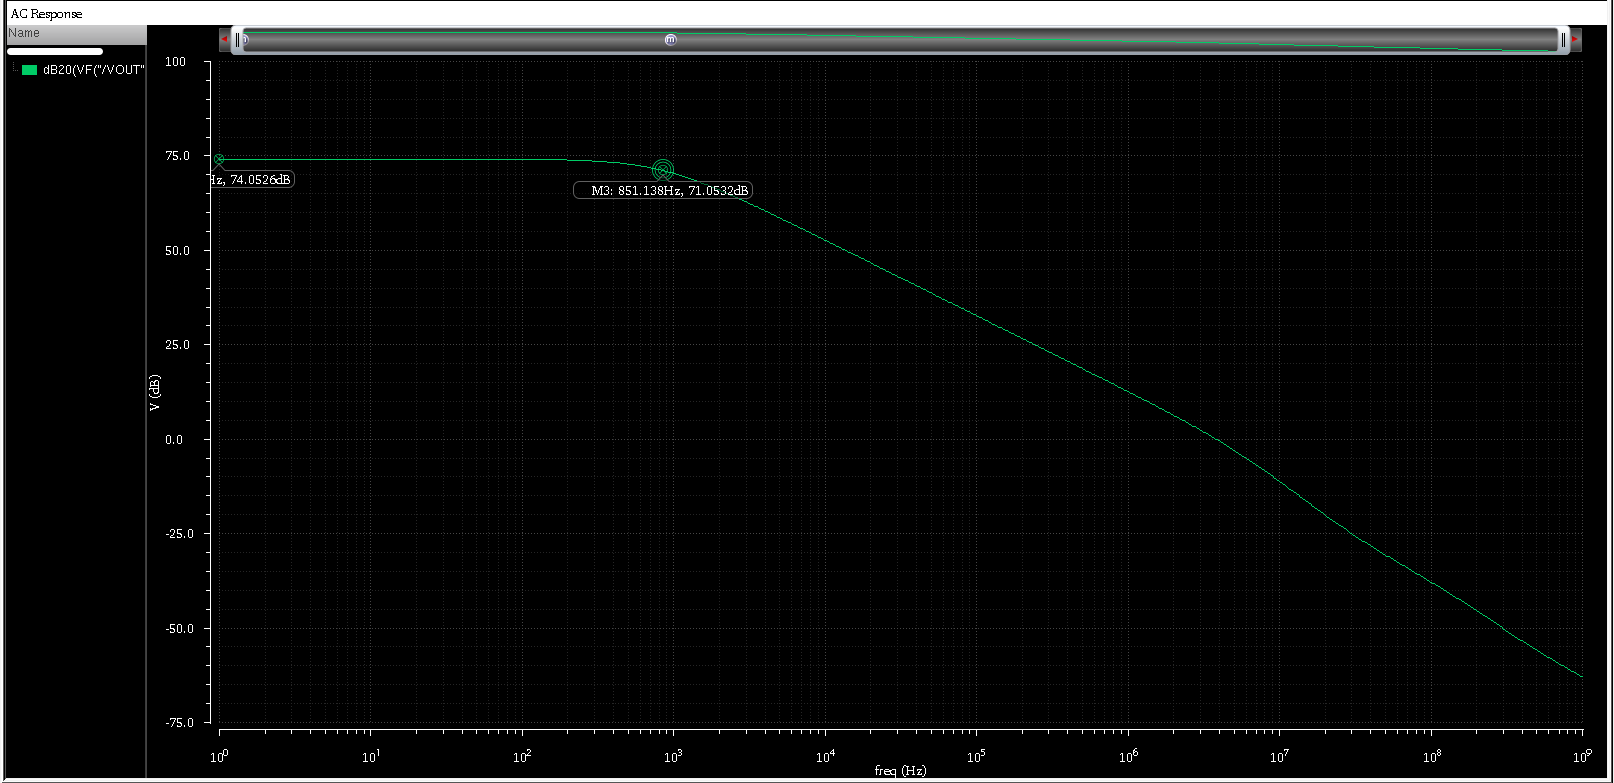
\includegraphics[width=\linewidth]{ad.png}
\caption{$A_d(0)=\SI{74.0526}{dB}$.}
\end{subfigure}\hfill
\begin{subfigure}[t]{0.49\textwidth}\centering
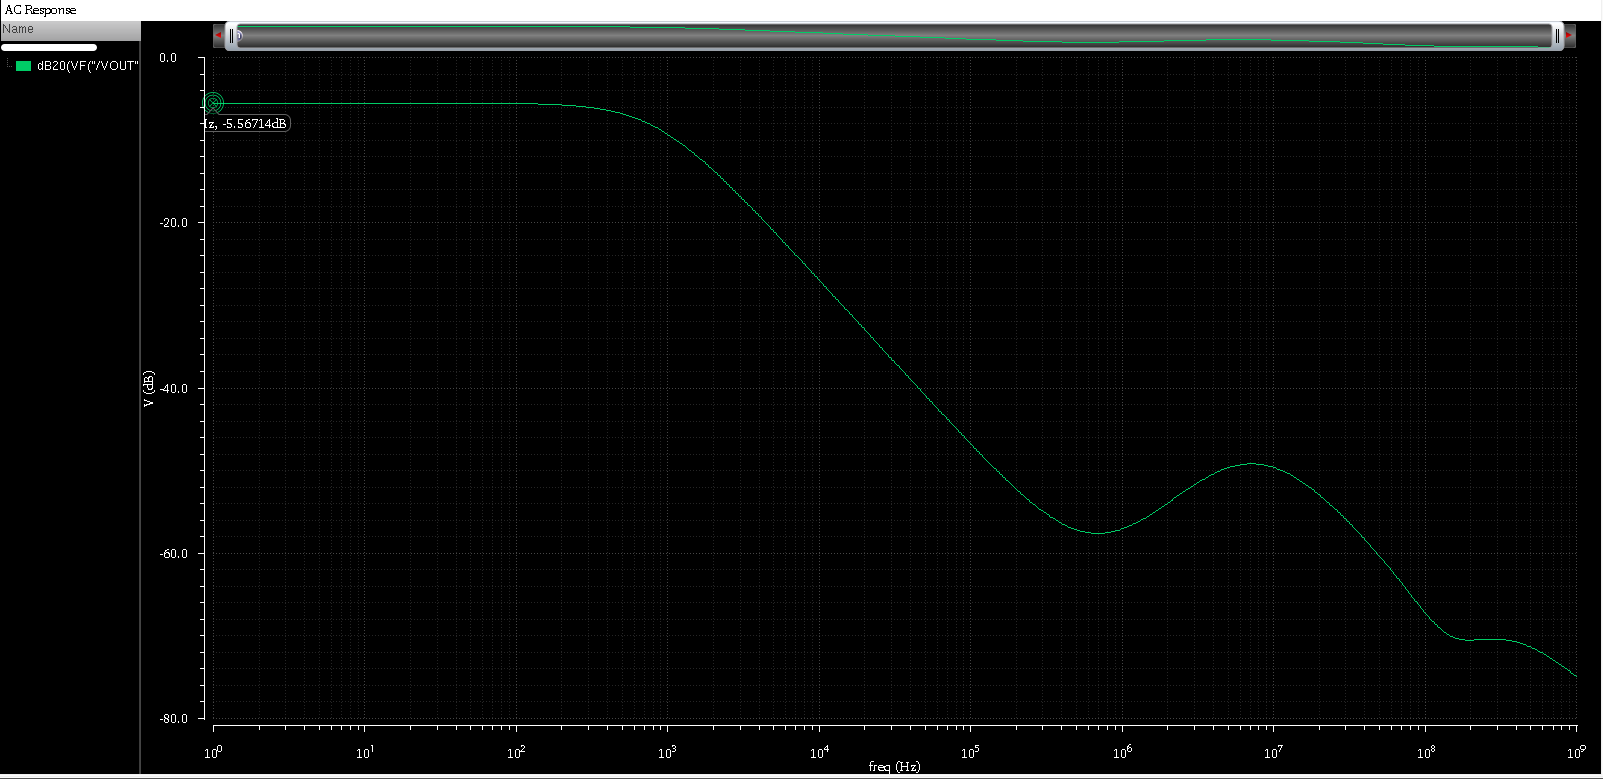
\includegraphics[width=\linewidth]{acm.png}
\caption{$A_{cm}(0)=\SI{-5.56714}{dB}$.}
\end{subfigure}
\caption{Differential and common-mode ac responses.}
\end{figure}

Therefore,
\begin{equation}
CMRR(0)=74.0526-(-5.56714)=\boxed{\SI{79.62}{dB}}.
\end{equation}
It is important not to label the \SI{74.05}{dB} differential-gain plot itself as CMRR; both $A_d$ and $A_{cm}$ are required.

\section{Power-supply rejection}
For PSRR$^+$, a \SI{1}{V} ac signal is applied to $V_{DD}$ while the signal inputs remain at their dc common-mode level and $V_{SS}$ is ac grounded. For PSRR$^-$, the injection is applied to $V_{SS}$ while $V_{DD}$ is ac grounded. With unity ac injection,
\begin{equation}
PSRR^{\pm}_{dB}=A_{d,dB}-20\log_{10}\left|\frac{V_{OUT}}{V_{SUPPLY}}\right|.
\end{equation}

\begin{figure}[H]\centering
\begin{subfigure}[t]{0.48\textwidth}\centering
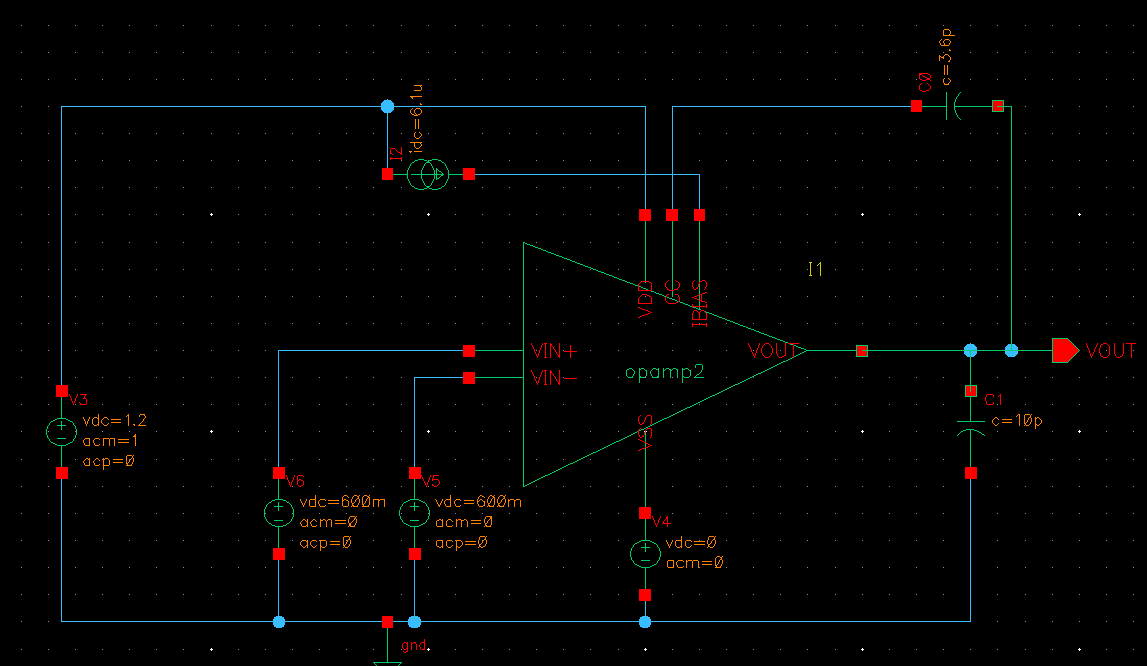
\includegraphics[width=\linewidth]{tb_psrr_plus.png}
\caption{PSRR$^+$ testbench.}
\end{subfigure}\hfill
\begin{subfigure}[t]{0.48\textwidth}\centering
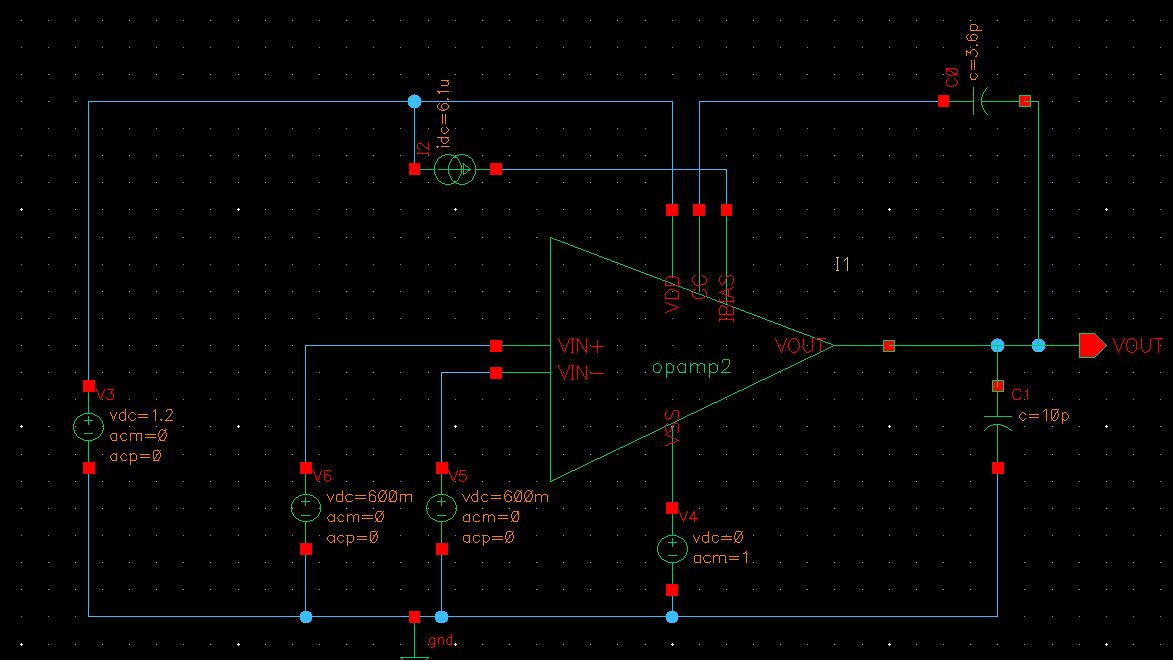
\includegraphics[width=\linewidth]{tb_psrr_minus.png}
\caption{PSRR$^-$ testbench.}
\end{subfigure}
\caption{Supply-ripple injection configurations.}
\end{figure}

\begin{figure}[H]\centering
\begin{subfigure}[t]{0.49\textwidth}\centering
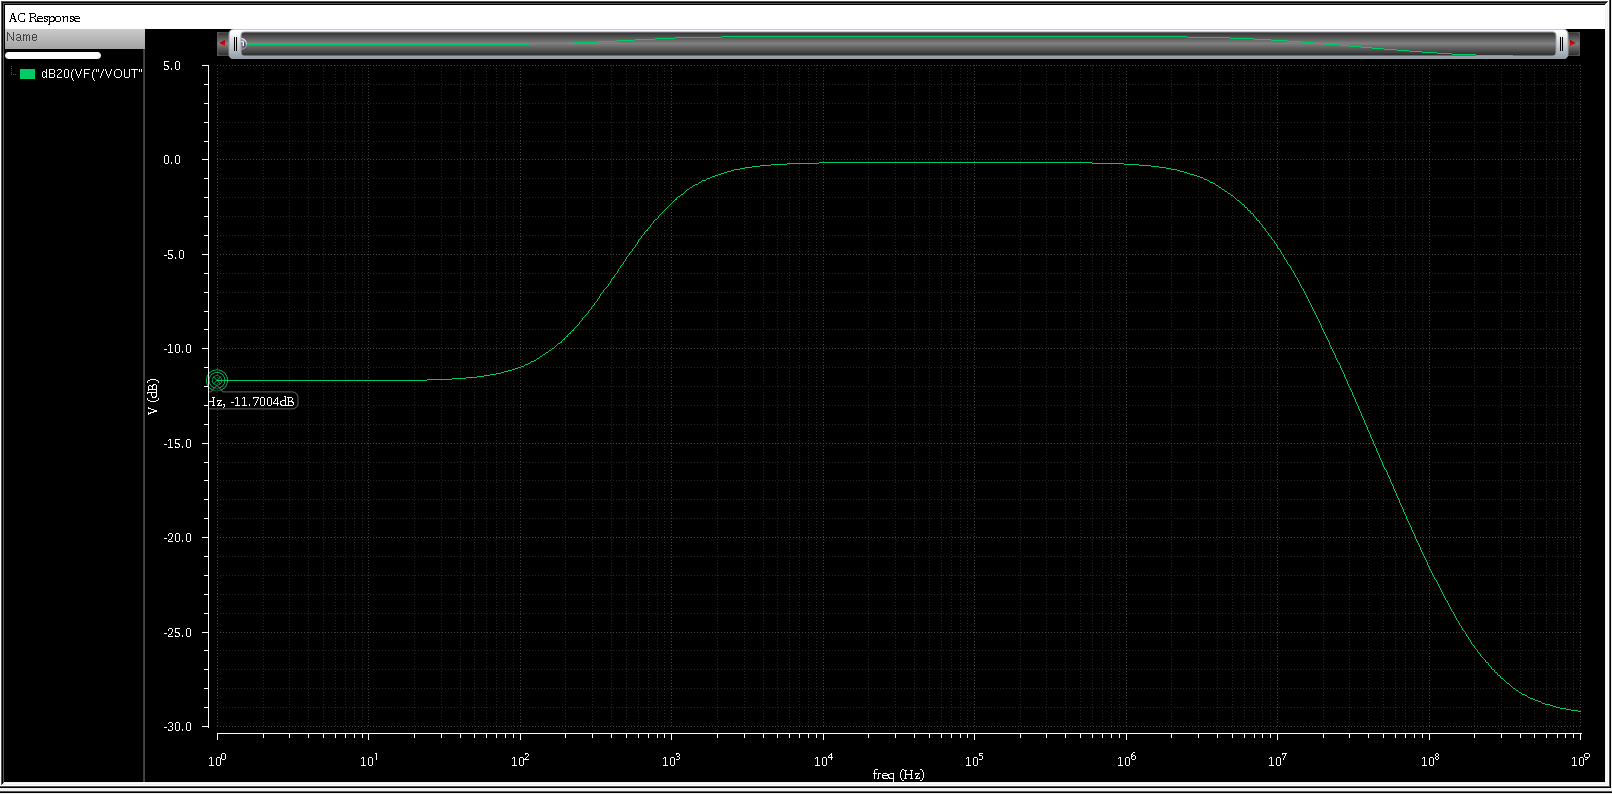
\includegraphics[width=\linewidth]{psrr_plus.png}
\caption{$A_{VDD}(0)=\SI{-11.7004}{dB}$.}
\end{subfigure}\hfill
\begin{subfigure}[t]{0.49\textwidth}\centering
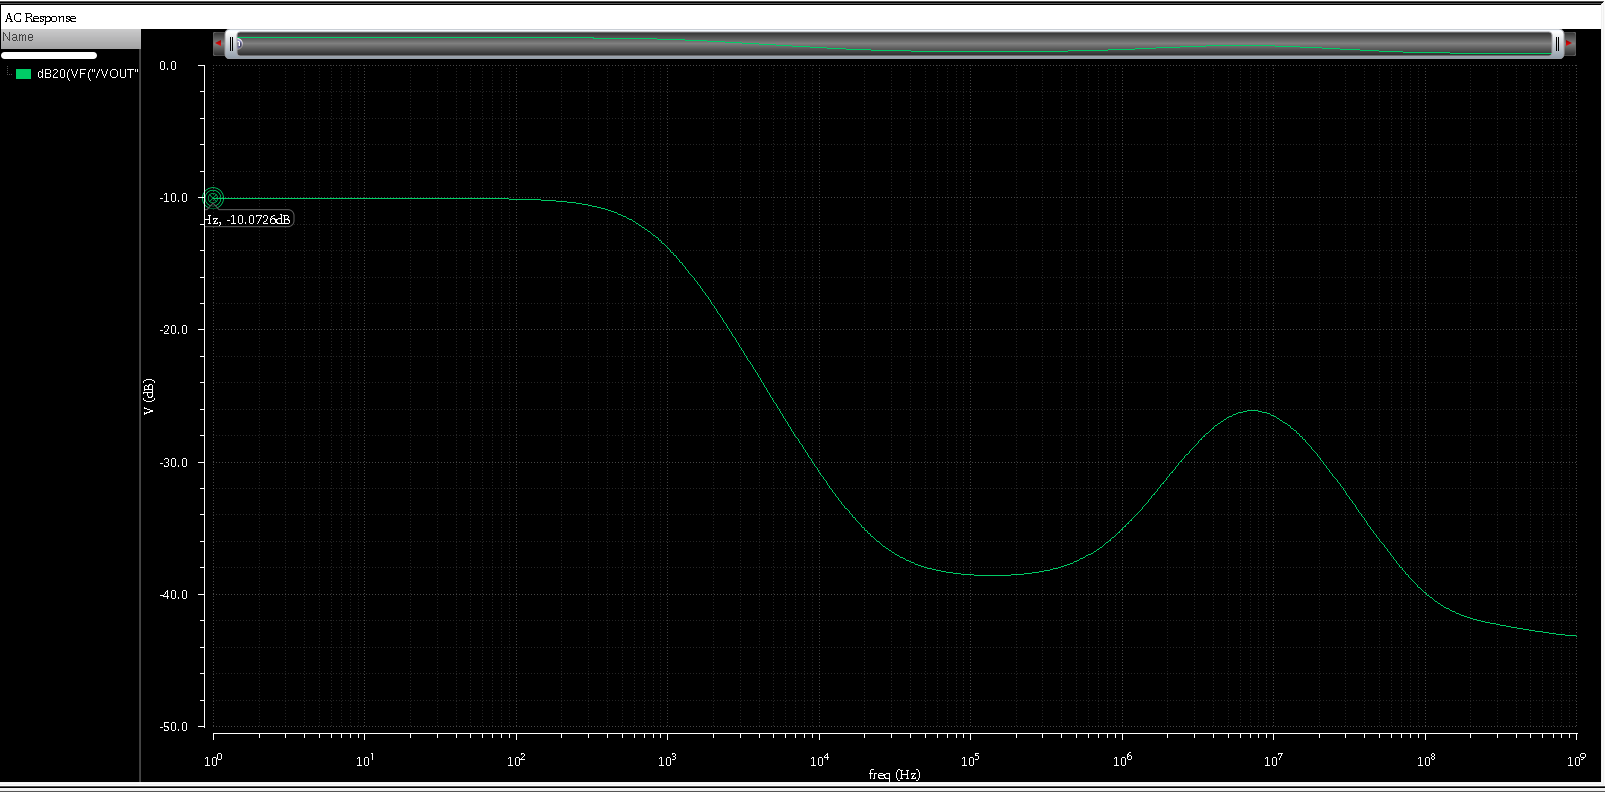
\includegraphics[width=\linewidth]{psrr_minus.png}
\caption{$A_{VSS}(0)=\SI{-10.0726}{dB}$.}
\end{subfigure}
\caption{Supply-to-output transfer functions. These curves are not PSRR until subtracted from differential gain.}
\end{figure}

The low-frequency rejection values are
\begin{align}
PSRR^+(0)&=74.0526-(-11.7004)=\boxed{\SI{85.75}{dB}},\\
PSRR^-(0)&=74.0526-(-10.0726)=\boxed{\SI{84.13}{dB}}.
\end{align}
The rejection degrades with frequency because supply disturbances couple through device capacitances and because the open-loop differential gain rolls off.

\chapter{Transient Analysis}

\section{Unity-gain step response}
The amplifier is connected as a voltage follower and driven by a \SI{0.4}{V} step between \SI{0.4}{V} and \SI{0.8}{V}. The step stays inside the intended ICMR and the load is \SI{10}{pF}.

\figwide[0.98\textwidth]{settling.png}{Input and output step responses used to evaluate overshoot and 1\% settling time.}

For a final value of \SI{0.8}{V}, the 1\% band is \SIrange{0.796}{0.804}{V}. For a final value of \SI{0.4}{V}, it is \SIrange{0.396}{0.404}{V}. The markers show
\begin{align}
t_{s,+}&\approx\SI{1.220467}{\micro s}-\SI{1.000250}{\micro s}
=\boxed{\SI{0.220}{\micro s}},\\
t_{s,-}&\approx\SI{6.251002}{\micro s}-\SI{6.001000}{\micro s}
=\boxed{\SI{0.250}{\micro s}}.
\end{align}
Both are comfortably below the selected \SI{1}{\micro s} requirement. The positive edge exhibits a small overshoot, while the negative edge has a larger undershoot; this asymmetry is consistent with different sourcing and sinking paths.

\section{Slew rate}
The analytical value is
\begin{equation}
SR_{calc}=\frac{I_5}{C_C}=\frac{\SI{18}{\micro A}}{\SI{3.6}{pF}}
=\boxed{\SI{5}{V/\micro s}}.
\end{equation}
From the derivative plot supplied during simulation, the negative slew marker is approximately \SI{-3.97}{V/\micro s}, while the positive edge is approximately \SI{4.7}{V/\micro s}. These values are slightly below the ideal calculation because part of the available current charges internal capacitances and because the output stage is not an ideal current source. For final sign-off, the derivative plot should be saved with both positive and negative flat-slope markers visible.

\chapter{Results and Discussion}

\section{Specification summary}
\begin{table}[H]
\centering
\caption{Target versus nominal simulation.}
\begin{tabularx}{\textwidth}{>{\bfseries}l l l >{\raggedright\arraybackslash}X}
\toprule
Metric & Target & Result & Status / comment\\
\midrule
DC gain & $\ge\SI{70}{dB}$ & \SI{74.05}{dB} & \pass; margin of \SI{4.05}{dB}\\
Unity-gain frequency & \SI{5}{MHz} & $\approx\SI{3.72}{MHz}$ & \fail; exact 0-dB marker should be added\\
Phase margin & $\ge\ang{60}$ & $\approx\ang{54.3}$ & \fail; stable but limited margin\\
Dominant-pole bandwidth & --- & \SI{851.14}{Hz} & Informational\\
Slew rate & \SI{5}{V/\micro s} & $+\approx4.7$, $-\approx3.97$ \si{V/\micro s} & \fail; analytical value is \SI{5}{V/\micro s}\\
1\% settling time & $\le\SI{1}{\micro s}$ & \SI{0.220}{\micro s}/\SI{0.250}{\micro s} & \pass\\
ICMR & \SIrange{0.4}{0.9}{V} & upper $\approx\SI{0.958}{V}$ & \pending; lower sweep has wrong mV range\\
Output swing & maximize & $\approx\SIrange{0.01}{1.10}{V}$ & \SI{1.09}{Vpp}, no-load dc\\
CMRR, low frequency & --- & \SI{79.62}{dB} & Calculated from $A_d-A_{cm}$\\
PSRR$^+$, low frequency & --- & \SI{85.75}{dB} & Calculated from $A_d-A_{VDD}$\\
PSRR$^-$, low frequency & --- & \SI{84.13}{dB} & Calculated from $A_d-A_{VSS}$\\
Quiescent output & near mid-supply & \SI{0.598}{V} & \pass\\
Estimated dc power & --- & \SI{154.5}{\micro W} & Analytical estimate, not supply-current measurement\\
\bottomrule
\end{tabularx}
\end{table}

\section{Main tradeoffs}
The final circuit is functional and fast in closed loop, but the gain, unity-gain frequency, phase margin, and negative slew rate do not reach their nominal targets simultaneously. The main tradeoffs are:
\begin{itemize}[leftmargin=18mm]
  \item Reducing $C_C$ raises GBW and slew rate, but generally reduces phase margin.
  \item Increasing $g_{m1}$ raises GBW but requires more input-stage current or larger M1--M2 devices, increasing power or capacitance.
  \item Increasing $g_{m6}$ improves non-dominant-pole separation, but raises second-stage current and may worsen the RHP-zero effect.
  \item A series nulling resistor $R_z\approx1/g_{m6}$ can remove or move the RHP zero. With $g_{m6}\approx\SI{551}{\micro S}$, $1/g_{m6}\approx\SI{1.81}{k\ohm}$. This can recover phase margin while allowing a smaller $C_C$, but must be re-simulated across corners.
  \item Longer channel lengths can increase intrinsic gain by reducing $g_{ds}$, but normally reduce speed and increase area.
\end{itemize}

\section{Required final checks}
Before tape-out-quality sign-off, the following simulations should be added:
\begin{enumerate}[leftmargin=18mm]
  \item repeat the lower ICMR sweep over \SIrange{0.2}{0.6}{V};
  \item place an exact 0-dB marker and read phase at that same frequency;
  \item save positive and negative derivative markers for slew rate;
  \item measure total supply current directly and report $P_{DC}=V_{DD}I_{DD}$;
  \item extract output resistance using a small-signal current injection at the output;
  \item run input-referred noise analysis, because noise is not present in the available result set;
  \item perform PVT and Monte Carlo mismatch analysis, particularly for gain, ICMR, output quiescent voltage, CMRR, and phase margin.
\end{enumerate}

\chapter{Conclusion}
An eight-transistor, two-stage Miller-compensated CMOS operational amplifier was designed in GPDK090 for a \SI{1.2}{V} supply and a \SI{10}{pF} load. The calculation flow produced a consistent initial bias and sizing set, including $I_5=\SI{18}{\micro A}$, $S_5=11.18$, and $S_8=3.79$. The dc operating point confirms balanced differential currents, balanced output-stage currents, saturation-region operation, and a quiescent output close to mid-supply.

The nominal simulation demonstrates useful performance: \SI{74.05}{dB} dc gain, approximately \SI{3.72}{MHz} unity-gain frequency, approximately \ang{54.3} phase margin, sub-\SI{0.3}{\micro s} 1\% settling, about \SI{1.09}{Vpp} no-load output swing, \SI{79.62}{dB} CMRR, and more than \SI{84}{dB} low-frequency PSRR. The revised dc-gain requirement of at least \SI{70}{dB} is satisfied with \SI{4.05}{dB} margin. The \SI{5}{MHz}, \ang{60}, and \SI{5}{V/\micro s} targets are not all met. The most direct next iteration is to increase second-stage transconductance and consider a Miller nulling resistor so that GBW can be raised without sacrificing phase margin. The lower ICMR must also be re-simulated with the correct voltage sweep before it is claimed as a verified result.

\begin{thebibliography}{9}
\bibitem{razavi}
B. Razavi, \emph{Design of Analog CMOS Integrated Circuits}, 2nd ed., McGraw-Hill Education, 2017.

\bibitem{baker}
R. J. Baker, \emph{CMOS: Circuit Design, Layout, and Simulation}, 3rd ed., Wiley-IEEE Press, 2010.

\bibitem{allen}
P. E. Allen, \emph{CMOS Analog Circuit Design: Design Procedure for the Unbuffered Two-Stage CMOS Operational Amplifier}, course lecture material, 2016.

\bibitem{cadence}
Cadence Design Systems, \emph{Virtuoso Analog Design Environment and Spectre Circuit Simulator}, simulation environment used for this project.

\bibitem{gpdk}
GPDK090 BSIM3 MOSFET models, nominal-corner transistor models used in the schematic simulations.
\end{thebibliography}

\appendix
\chapter{Measurement Definitions}
\begin{align}
A_{d,dB}(f)&=20\log_{10}\left|\frac{V_{OUT}}{V_{ID}}\right|,\\
A_{cm,dB}(f)&=20\log_{10}\left|\frac{V_{OUT}}{V_{ICM}}\right|,\\
CMRR_{dB}(f)&=A_{d,dB}(f)-A_{cm,dB}(f),\\
PSRR^+_{dB}(f)&=A_{d,dB}(f)-20\log_{10}\left|\frac{V_{OUT}}{V_{DD,ac}}\right|,\\
PSRR^-_{dB}(f)&=A_{d,dB}(f)-20\log_{10}\left|\frac{V_{OUT}}{V_{SS,ac}}\right|,\\
SR_+&=\max\left(\frac{\dd V_{OUT}}{\dd t}\right),\qquad
SR_-=\min\left(\frac{\dd V_{OUT}}{\dd t}\right).
\end{align}
For settling time, the start time is the input's 50\% crossing and the stop time is the final entry into the specified error band without any later excursion.

\end{document}
